\label{chap:algorithm_selection}
As introduced in Chapter \ref{chap:introduction}, the local search-based heuristics are the main focus in this work.
In this chapter, the local search algorithm along with its local optimum problem is discussed first. Then, the two typical
local search-based heuristics, simulated annealing and tabu search, are represented. Last, the most promising algorithm is
proposed to the memory power optimization according to the comparison between these heuristics.

	\section{Local search algorithm}
	\label{sec:local_search}
	Local search algorithm is one of the simplest heuristics. Given a optimization problem, it starts from an initial solution
	and searches in the current solution's neighborhood. If a better solution is found, the current solution is replaced by it. 
	The searching process is repeated until there is no better solution in the current solution's neighborhood. Then it outputs 
	the current solution as the algorithm result.
	Algorithm \ref{algo:local_search} shows the pseudo-code of local search process. There are four main steps in the algorithm.
	First step is finding a initial solution and set it as the current solution. The initial solution should be valid for the problem.
	In the second step, a neighboring solution is generated by certain mechanism. And the third step is to compare the neighboring
	solution with the current one through a object function. The object function is a method to indicate how good the solution is.
	The last step is the selection criterion for solution. Local search algorithm selects the better one between the current and neighboring solution, which is a naive criterion.
		
	\begin{algorithm2e}[H]
	\KwData{an optimization problem}
	\KwResult{an optimal solution}
	current solution = initial solution\;
	\While{not terminate}
	{
		generate a neighboring solution\;
		evaluate the neighboring solution\;
		\If{neighboring solution is better than current solution}
		{
			current solution = neighboring solution\;
		}
	}
	output current solution\;
	\caption{Local Search Algorithm}
	\label{algo:local_search}
	\end{algorithm2e}
	
	Though local search algorithm is simple, the solution it provides may be the local optimal one. This is the major problem of
	local search algorithm. Figure \ref{fig:local_optimum_local_search} illustrates this local optimum trap. Suppose the
	optimization problem is to find the solution with minimum cost, the local search algorithm starts with the initial solution $a$.
	The cost of neighboring solution $b$ is lower than cost of $a$, then $b$ becomes the current solution. The same searching process 
	is repeated until the current solution reaches $c$. There is no better solution in $c$'s neighborhood, thus the algorithm outputs solution $c$ and terminates. However, solution $c$ is only the local optimum and the global optimum is solution $e$ which
	is not in $c$'s neighborhood. In order to reach solution $e$, the algorithm has to move to solution $d$ whose cost is higher than
	$c$'s cost. And this violates the selection criterion of the algorithm. Another drawback of local search algorithm is that the result quality is dependent on the initial solution. If the algorithm starts with solution $d$, the output will be the global optimum $e$. These two disadvantages make local search algorithm an improper choice when global optimal solution is required for 
	the optimization problems. 
	
	\begin{figure}[H]
		\begin{center}
			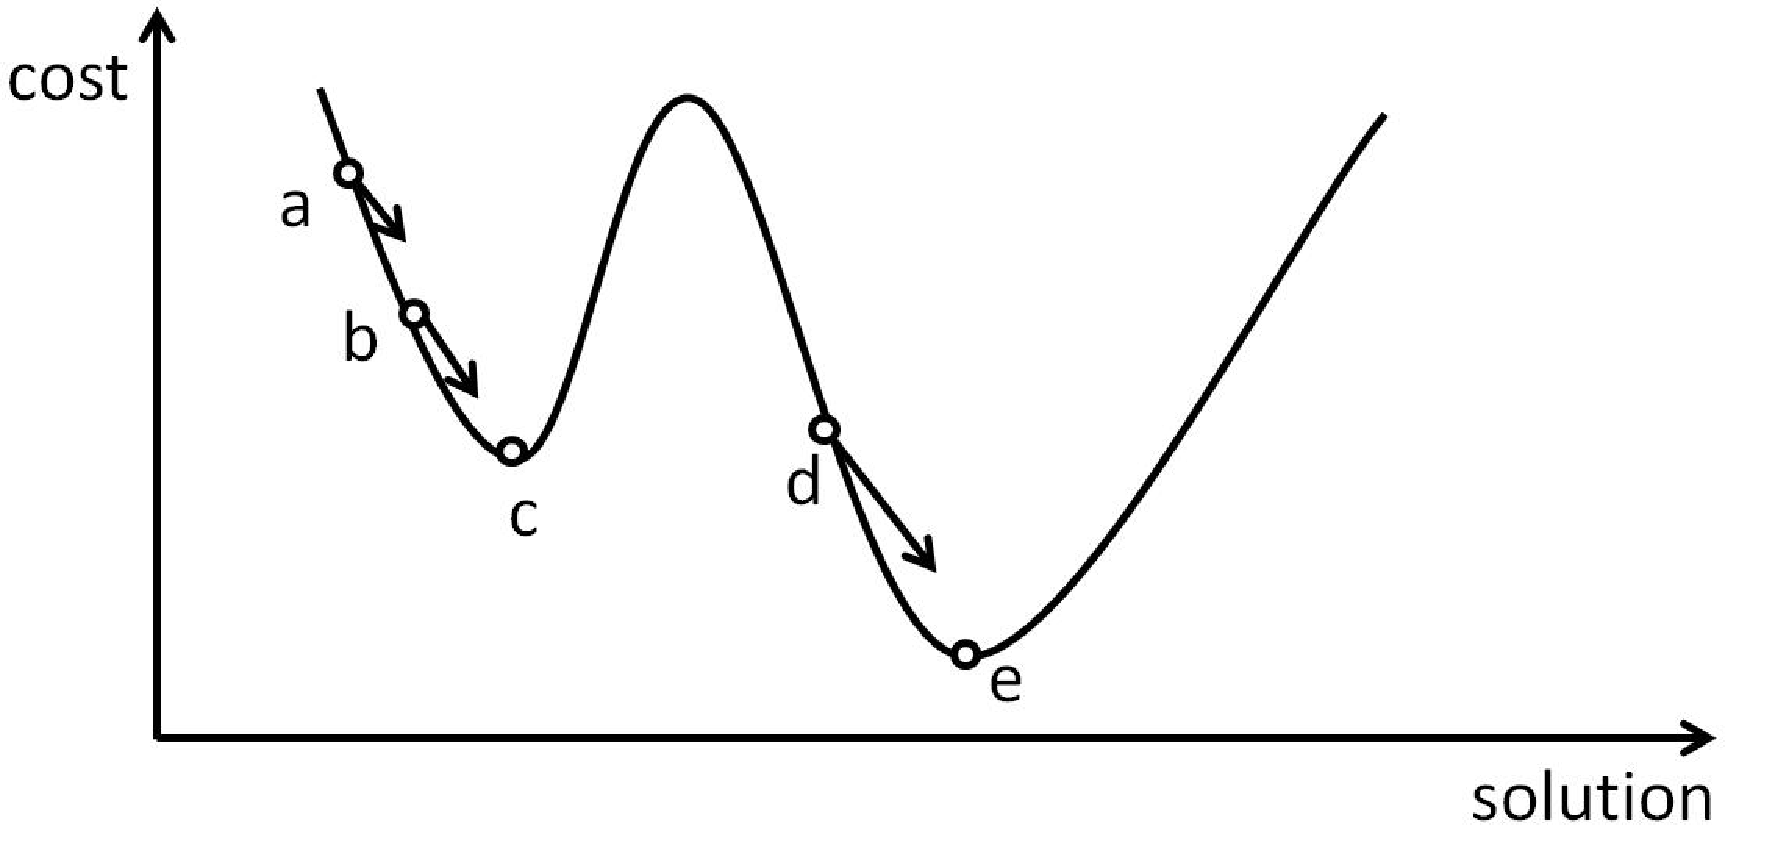
\includegraphics[width=0.7\textwidth]{local_optimum_local_search}
			\caption[Local Optimum Problem]{Local Optimum Trap}
			\label{fig:local_optimum_local_search}
		\end{center}
	\end{figure}


	\section{Tabu search algorithm}
	\label{sec:tabu_search}
	One of the improvements to local search is the tabu search algorithm. It is based on the local search but it avoids to
	stuck at the local optimum trap through a different selection criterion for solutions. As discussed in chapter \ref{sec:local_search}, once the local search algorithm is trapped at a local optimal solution, it cannot move any further due to the naive solution selection criterion.  
	
	
	
	